\section{Appendix}
Hier wird der zusätzliche Content abgebildet.

\subsection{Ältere Versionen des Komponentendiagramms}
Hier werden die älteren Versionen und Entwürfe des Komponentendiagramms abgelegt.

\subsubsection{Komponentendiagramme}
Im folgenden sind die älteren Versionen unserer Komponentendiagramme

\begin{figure}[H]
\centering
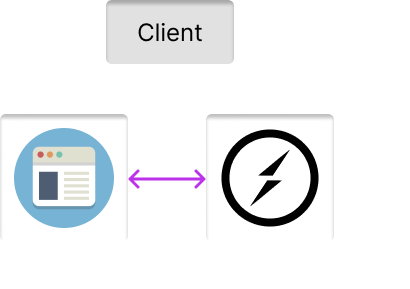
\includegraphics[width=0.5\textwidth]{bilder/technologien/KomponentendiagramClient.png}
\caption{Komponentendiagramm Client}
\label{fig:Komponentendiagramm_Client}
\end{figure}
\noindent Hier wird die Client Seite bildlich dargestellt. Man sieht, dass der Webbrowseer durch die 
Socket.io Client deployed wird und dadurch wird dann eine Beziehung zur Serverseite aufgebaut. (Siehe Abbildung \ref{fig:Komponentendiagramm_Client})

\begin{figure}[H]
\centering
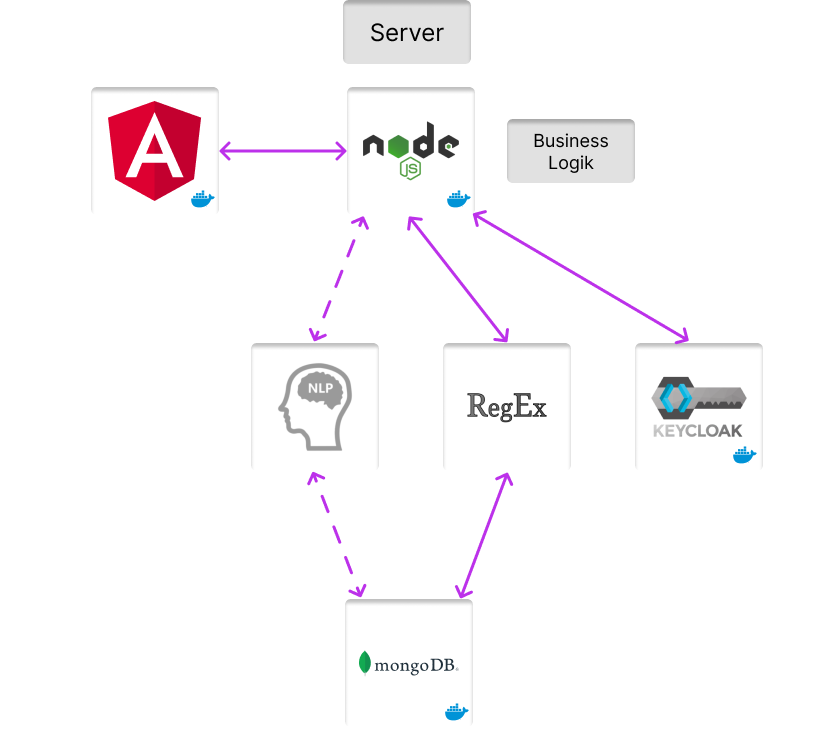
\includegraphics[width=0.9\textwidth]{bilder/technologien/KomponentendiagramServer.png}
\caption{Komponentendiagramm Server}
\label{fig:Komponentendiagramm_Server}
\end{figure}

\noindent In der Serverseite wird dann durch den Socket.io Server die Verbindug zum Clienten aufrecht gehalten.
Im Server befindet sich Angular, node.js, KeyCloak und die Datenbank mongoDB und haben jeweils einen eigenen Dockercontainer. 
Die Erkennung von der eingegeben Sprache möchten wir zunächst mit RegEx ermöglichen, 
um das Minimal Viable Product hinzubekommen. Optional dann mit NLP (Natural Language Processing) erweitern.

\begin{figure}[!hbt]
    \centering
    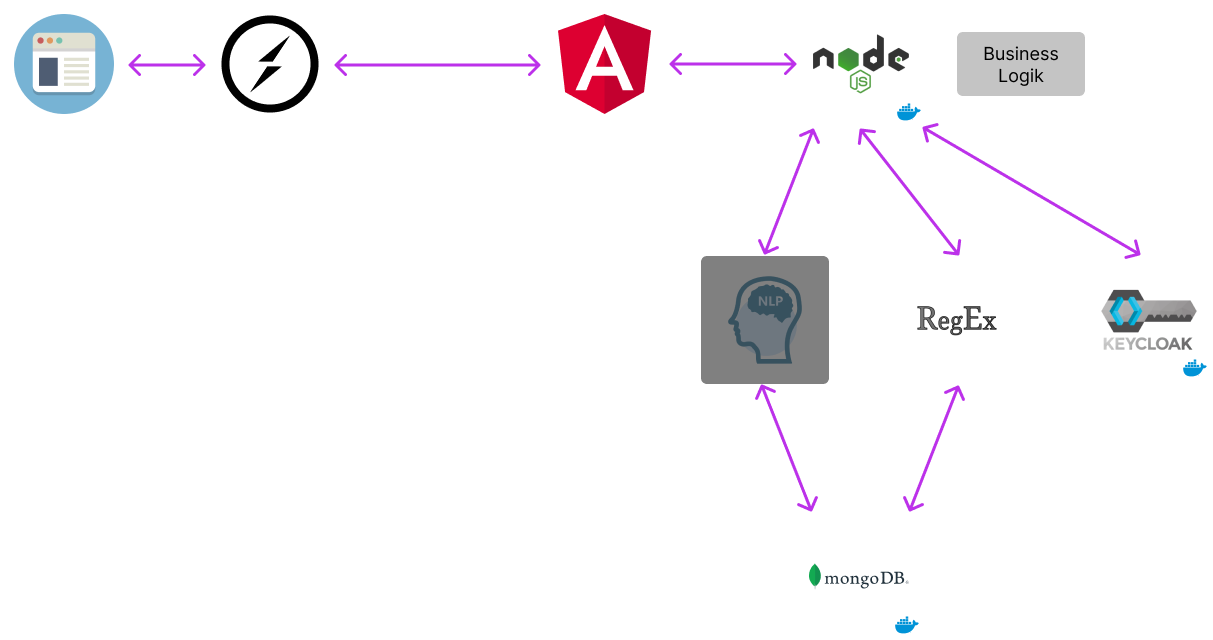
\includegraphics[width=1.0\textwidth]{bilder/technologien/Komponenten-Diagram-v1.png}
    \caption{Komponentendiagramm v1.0}
    \label{fig:Komponentendiagramm_v1.0}
    \end{figure}

\noindent In dieser Version haben wir erst einmal die Struktur von unseren Komponentengesucht und eine
grobe Darstellung erstellt. Was wir hier aber nicht wussten ist, wie wir das NLP darstellen sollten.
NLP war für uns vorher eine optionale Möglichkeit.

    \begin{figure}[!hbt]
        \centering
        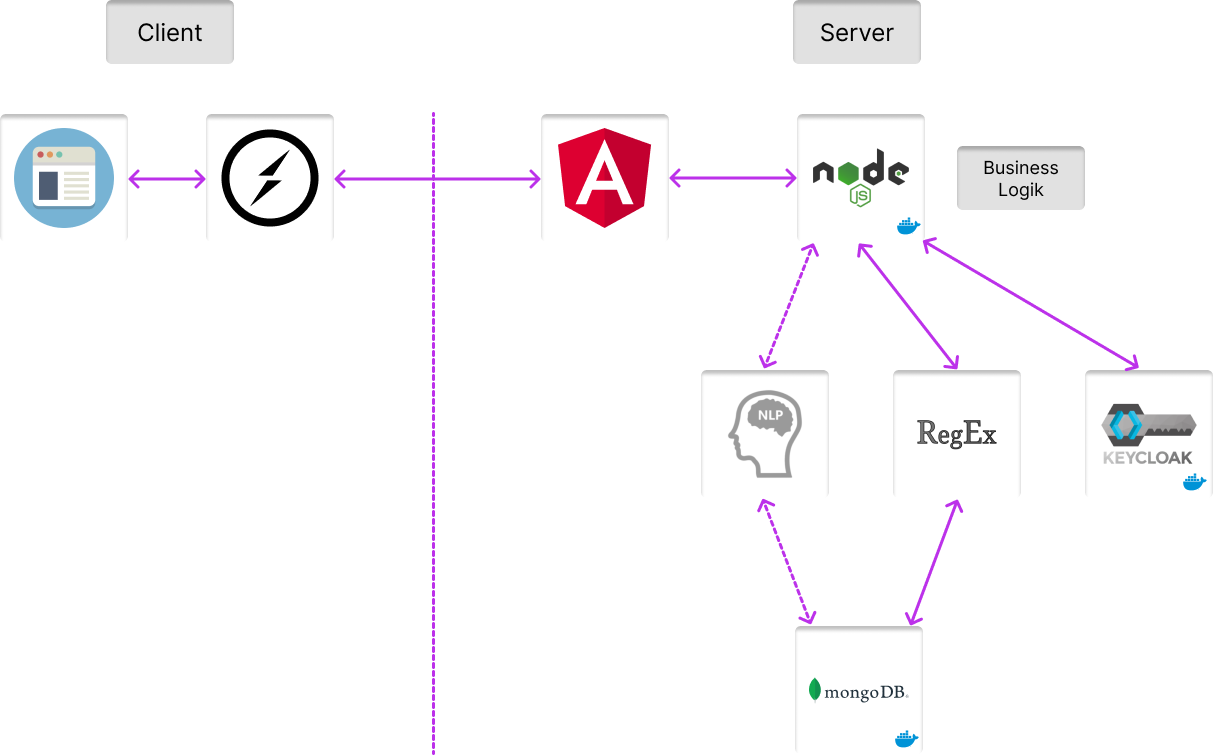
\includegraphics[width=1.0\textwidth]{bilder/technologien/Komponentendiagram v1.1.png}
        \caption{Komponentendiagramm v1.1}
        \label{fig:Komponentendiagramm_v1.1}
        \end{figure}
        \FloatBarrier 

\noindent In dieser Darstellung haben wir die einzelnen Komponenten in Server und Client 
eingeteilt, um die Struktur besser zu verstehen. Wir haben aber die Abtrennung nicht richtig anzeigen können
und das NLP haben wir auch nicht klar als optional zeigen können.

    \begin{figure}[!hbt]
        \centering
        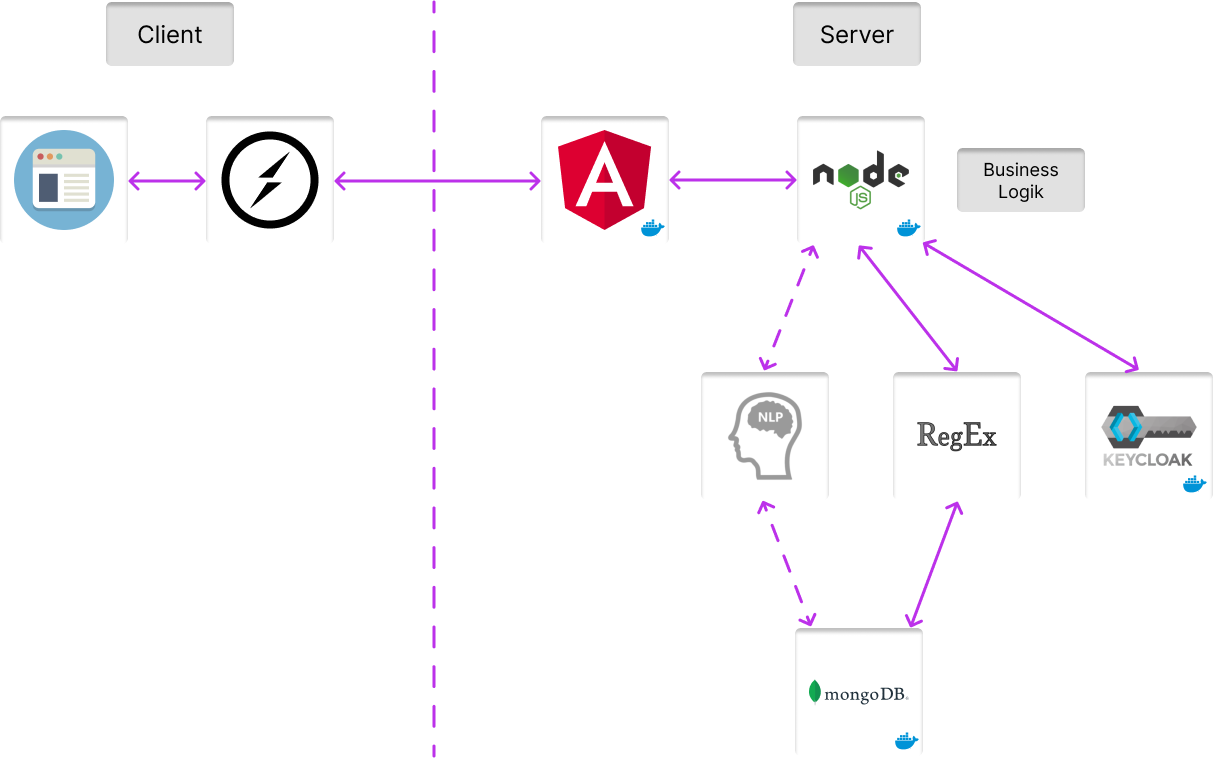
\includegraphics[width=1.0\textwidth]{bilder/technologien/Komponentendiagram v1.2.png}
        \caption{Komponentendiagramm v1.2}
        \label{fig:Komponentendiagramm_v1.2}
        \end{figure}
        \FloatBarrier % prevent pictures from appearing under a different section
    